
\documentclass[
  english,        % define the document language (english, german)
  font=times,     % define main text font (helvet, times, palatino, libertine)
  onecolumn,      % use onecolumn or twocolumn layout
]{tumarticle}


% load additional packages
\usepackage{lipsum}
\usepackage{csquotes}
\usepackage[style=numeric-comp,sorting=none]{biblatex}
\usepackage{graphicx}
\usepackage{amsmath}
\usepackage{subcaption}

\addbibresource{resources/literature.bib}


% article metadata
\title{Time stepping review of open-source solvers}
\subtitle{Guided research}

\author[email=marc.amoros@tum.de]{Marc Amorós}

\date{
    \small
    \textbf{Supervisor:} Prof. Dr. Hans-Joachim Bungartz \\
    \textbf{Advisor:} M.Sc. Benjamin Rodenberg \\
}

\begin{document}

\maketitle

\begin{abstract}
    The accurate numerical simulation of physical phenomena is crucial in various scientific and engineering disciplines, and open-source solvers offer flexibility and accessibility to research and practitioners. A vital aspect of these solvers is the order of the time stepping scheme employed to evolve the solution over time, as it significantly affects the error of the obtained solutions. This work investigates and verifies the order of different time stepping methods implemented on various solvers. We focused on higher-order methods, which give better accuracy and help reduce the computational costs of obtaining a precise enough solution. To inspect the order of fluid-structure interaction (FSI) simulations using preCICE, we chose OpenFOAM and CalculiX as the studied solvers, which are compatible with this coupling library. 

    We observed a higher-order convergence when using second-order methods in single-solver simulations on both solvers and confirmed the correct convergence of first-order methods on FSI simulations. Moreover, we tested higher-order time stepping schemes on FSI simulations, which gave sub-linear error convergence. We followed by ruling out possible causes of this poor convergence and proposing possible solutions, making this work valuable for future projects aiming to obtain accurate FSI simulations in the preCICE environment.
\end{abstract}

\section{Introduction}
In scientific and engineering simulations, the precise numerical representation of physical phenomena is crucial for advancing knowledge and solving practical challenges. Open-source solvers have emerged as indispensable tools, offering flexibility and accessibility to researchers and practitioners alike. These solvers offer different time stepping schemes, and selecting one to evolve the solution over time is a decision that profoundly influences the error of the obtained solutions. This project investigates and verifies various time stepping methods implemented on different open-solvers, focusing on higher-order schemes.
    
Higher-order methods not only promise enhanced accuracy but also hold the potential to mitigate computational costs, which is crucial for obtaining precise solutions within reasonable time frames. Our study analyses if these claims hold for two specific open-source solvers and presents scenarios where higher-order convergence can be achievable. 

One can differentiate between single or multi-physics simulations. The first group target a specific domain, such as fluid dynamics, structural mechanics, heat transfer, or electromagnetics. The solvers of said simulations focus on solving equations specific to their respective domains and are often tailored to efficiently handle the complexities of that particular physics. On the other hand, multi-physics solvers integrate multiple physical domains into a single simulation framework. 

We selected OpenFOAM \cite{weller1998tensorial} and CalculiX \cite{calculix-web} as our fluid mechanics and structural solvers, respectively, given that they are widely used in industry and research, renowned for their reliability and good documentation. Moreover, both are compatible with the multi-physics coupling library preCICE \cite{preCICEv2}, which allowed us to compute fluid-structure interaction (FSI) simulations using both solvers as black boxes. This way, we could combine fluid dynamics and structural mechanics solvers to predict the dynamic behavior of structures immersed in fluid flows.

In the subsequent sections, we show how higher-order convergence is achievable in single-solver simulations using second-order methods. Furthermore, we couple the two single-physics solvers in an FSI simulation and observe how a linear convergence can be achieved with first-order time stepping methods. Contrarily, we display how using a second-order method does not improve but worsens the error convergence.

For transparency and reproducibility, all code utilized in this project is accessible via our repository at: \url{https://github.com/atmarc/guided_research}. 

\section{OpenFOAM}
OpenFOAM is an open-source computational fluid dynamics (CFD) software package widely used for simulating and analyzing complex fluid flow problems. Its solver modules employ finite volume methods to numerically solve the Navier-Stokes equations, making it a versatile tool for simulating fluid dynamics in various engineering and scientific applications. In this section, we will explain the convergence analysis performed to verify that it has a higher-order convergence in time.   

\subsection{Time stepping schemes}\label{sec:euler}
This solver offers various time stepping schemes, and we focused on two for our analysis. The first one is the Euler implicit scheme. Given the following partial differential equation:

\begin{equation}
    \frac{\partial u}{\partial t} = F(u, t)
\end{equation}
the Euler implicit scheme would discretize it as follows:

\begin{equation}
    \frac{u^{n+1} - u^n}{\Delta t} = {F}(u^{n+1}, t^{n+1})
\end{equation}
it is a first-order method that is relatively stable, which is why it is usually the default choice. For the purpose of this study, we also chose a second-order scheme, this being the Crank-Nicolson method \cite{crank1947practical}. This scheme combines an explicit and an implicit Euler step, leading to a second-order convergence in time. This method would discretize the previous PDE as: 

\begin{equation}
    \frac{u^{n+1} - u^n}{\Delta t} = \frac{1}{2} \left[F(u^n, t^n) +  F(u^{n+1}, t^{n+1}) \right]
\end{equation}
OpenFOAM uses a slightly different version of this method by introducing a blending coefficient $\theta$ between the Euler implicit and Crank-Nicolson methods. If $\theta = 0$, then we obtain the implicit Euler method, and if $\theta = 1$, then it's Crank-Nicolson. For stability, the value $\theta = 0.9$ is recommended in their documentation.

\begin{equation}
    \frac{u^{n+1} - u^n}{\Delta t} = \frac{\theta}{2} F(u^{n}, t^{n}) + \left( 1 - \frac{\theta}{2} \right) F(u^{n+1}, t^{n+1})
\end{equation}


\subsection{Convergence study}

To study the convergence behaviour of OpenFOAM, we focused on the Taylor-Green vortex \cite{taylor1937mechanism, chorin1968numerical}, a standard setup in CFD to validate fluid flow solvers, given that an analytical solution of the case is known. In a 2D scenario, the solution can be obtained by the formulas:
\begin{align}
    &u(x, y, t) = -\cos(x) \sin(y) e^{-2\mu t} \\
    &v(x, y, t) = \sin(x) \cos(y) e^{-2\mu t} \\
    &p(x, y, t) = -\frac{1}{4}\left[\cos(2x) + \sin(2y)\right]e^{-2\mu t}
\end{align}
where $u$ and $v$ are the horizontal and vertical velocities respectively, $p$ is the pressure and $\mu$ is the viscosity of the fluid. This solution holds for a square domain of size $2\pi$. In Figure \ref{fig:taylor-green} we can see an example of the computed initial velocities. 

\begin{figure}[!ht]
    \centering
    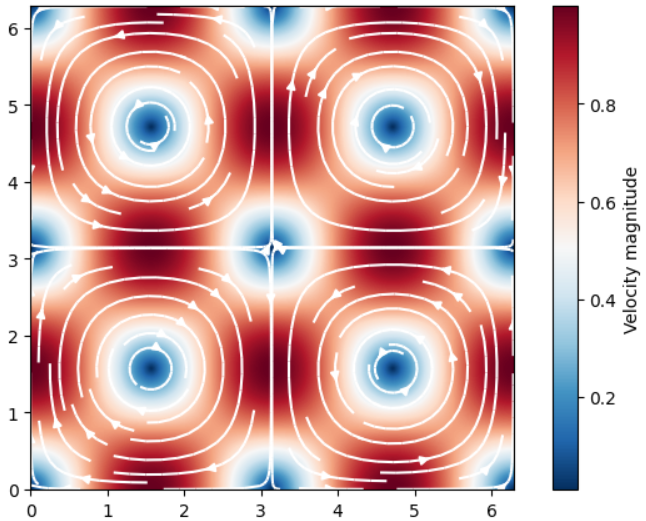
\includegraphics[width=0.5\textwidth]{resources/taylor-green-vortex.png}
    \caption{Visualization of the Taylor-Green vortex scenario.}
    \label{fig:taylor-green}
\end{figure}

We implemented a program that computes the initial velocity for this setup and writes it into the OpenFOAM configuration. We also wrote a script to automatize the configuration and execution of different setups with varying parameters so we can perform several experiments automatically.
We ran our setup case several times to observe the error behaviour, fixing all the parameters (grid size, initial velocity and solver tolerances) and changing the timestep size. In our analysis, we mainly focused on the velocity profile.

In a simulation, several elements contribute to the error $\varepsilon_{u}$. In this study, we were only interested in the error contribution of the time discretization scheme $\varepsilon_{\Delta t}$ to verify the order of the scheme. We assume that the error is formed by $\varepsilon_u = \varepsilon_{\Delta t} + \varepsilon_{\Delta x} + \varepsilon_\text{num}$, where $\varepsilon_{\Delta x}$ is the spatial discretization error, and $\varepsilon_\text{num}$ is the error introduced by numerical errors and other factors. We know that $\varepsilon_{\Delta x}$ is related to the grid size, so we can assume that it is constant among the experiments with the same grid size.

\begin{figure}[!htbp]
    \centering
    \begin{subfigure}[b]{0.49\textwidth}
      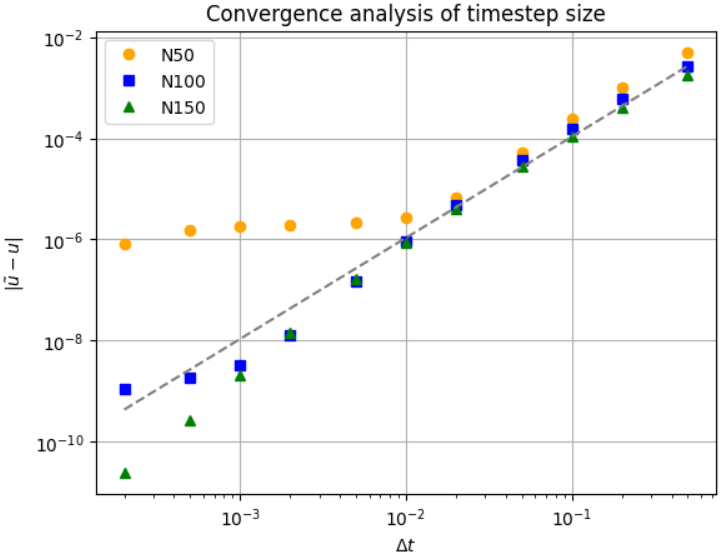
\includegraphics[width=\textwidth]{resources/convergence_study_openfoam.png}
      \caption{}
      \label{fig:convergence_openfoam}
    \end{subfigure}
    \hspace{1pt}
    \begin{subfigure}[b]{0.49\textwidth}
        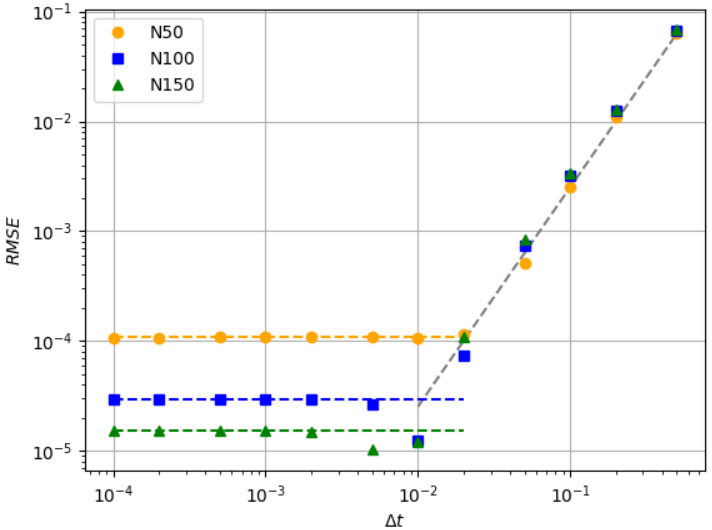
\includegraphics[width=\textwidth]{resources/RMSE_study.png}
      \caption{}
      \label{fig:RMSE_openfoam}
    \end{subfigure}
    \caption{Figure (a) shows the convergence study of the Taylor-Green vortex case, utilizing three different grid resolutions. The error is measured by comparing the fluid field value in a specific position with the reference solution ($\Delta t = 10^{-5}$). In Figure (b), we have the same convergence study but using the analytical solution as the reference value, and we plotted the RMSE in the y-axis.}
    \label{fig:figures}
  \end{figure}
  

There are several possible approaches to studying the error. Our first strategy was to choose a position cell $(i,j)$ and compare the cell values in this position for the different samples. We define the reference sample $\tilde{u}$, obtained by running the simulation with a $\Delta t = 10^{-5}$. 
We computed the absolute difference between every sample and the chosen reference solution $|u - \tilde{u}|$ and plotted them in Figure \ref{fig:convergence_openfoam} for three different grid sizes. The spatial error being constant among samples means that the plot is showing $\varepsilon_{\Delta t} + \varepsilon_\text{num}$, allowing us to extract conclusions from the convergence behaviour of $\varepsilon_{\Delta t}$. We can observe how the error decreases when the timestep gets smaller, proportionally to $\mathcal{O}(\Delta t^2)$, until the error flattens. We assume that this happens when $\varepsilon_{\Delta t} < \varepsilon_\text{num}$, and after a certain point, this $\varepsilon_\text{num}$ dominates the entire error. It is also remarkable to see how this point of flattening happens in smaller time steps when increasing the domain resolutions.
  
As mentioned before, the Taylor–Green vortex scenario has an analytical solution $u^*$, which allows us to obtain the exact error $\varepsilon_{u}$ of the solutions we obtained, as those are going to be of the form $u = u^* + \varepsilon_{u}$. To compute this error $\varepsilon_{u}$, we compute the root-mean-square error (RMSE) of the velocity flow field, compared to the analytical solution as follows:  

\begin{equation}
    \text{RMSE} = \sqrt{\sum_{(i,j)} (u^*_{ij} - u_{ij})^2 }
\end{equation}

This error is being plotted in Figure \ref{fig:RMSE_openfoam}, where we can observe the error decreasing proportionally to $\mathcal{O}(\Delta t^2)$, showing once again a second-order convergence in time. The flattening of the error is very visible in this plot after a specific timestep size. The plateau of the error occurs when $\varepsilon_{\Delta t} < \varepsilon_{\Delta x}$, as we include the spatial error in this scenario. This plot also clearly shows how this spatial error decreases for higher domain resolutions and gives a clear idea of its magnitude. 


\section{CalculiX}\label{sec:calculix}
CalculiX is an open-source finite element software suite primarily used for solving structural analysis problems. It is designed to simulate the behaviour of mechanical and structural systems subjected to various loading conditions. CalculiX provides capabilities for linear and nonlinear static, dynamic, and thermal analyses. It supports a variety of element types, boundary conditions, and material models, making it suitable for a wide range of engineering simulations. In this section, we will overview the time stepping scheme implemented in the solver and present the convergence study we performed, which displays a higher-order convergence. 

\subsection{Time stepping scheme}\label{sec:alpha}
The only time stepping scheme implemented in CalculiX is the $\alpha$-method \cite{dhondt2017calculix}. The solver allows the user to select between an implicit or an explicit version of it and allows to control the $\alpha$ parameter. Moreover, one can define a fixed timestep size using the DIRECT clause. To get an idea of how this method works, we can start with a given material point with displacement $\boldsymbol{u}$, velocity $\boldsymbol{v}$ and acceleration $\boldsymbol{a}$. We know that the acceleration and velocity are related as such $\boldsymbol{a} = \dot{\boldsymbol{v}}$, and this yields the following formula to obtain the following timestep values:
\begin{equation}
    \boldsymbol{v}^{n+1} = \boldsymbol{v}^n + \int_{t^n}^{t^{n+1}} \boldsymbol{a(\xi)} \text{d}\xi
\end{equation}
The integral on the right-hand side can be approximated by a linear combination of $ \boldsymbol{a}^n$ and $\boldsymbol{a}^{n+1}$:
\begin{gather}
    \boldsymbol{a}(\xi) \approx  (1 - \gamma) \boldsymbol{a}^n + \gamma \boldsymbol{a}^{n+1}\\
    \boldsymbol{v}^{n+1} = \boldsymbol{v}^n + \Delta t \left[ (1 - \gamma) \boldsymbol{a}^n + \gamma \boldsymbol{a}^{n+1} \right]
\end{gather} 
A similar reasoning can be applied to $\boldsymbol{u}$, as $\boldsymbol{\dot{u}} = \boldsymbol{v}$, hence:
\begin{equation}
    \boldsymbol{u}^{n+1} 
    = \boldsymbol{u}^n + \int_{t^n}^{t^{n+1}} \boldsymbol{v(\eta)}  \text{d}\eta 
    = \boldsymbol{u}^n + \Delta t \boldsymbol{v}^n + \int_{t^n}^{t^{n+1}} \int_{t^n}^{\eta} \boldsymbol{a(\xi)} \text{d}\xi \text{d}\eta 
\end{equation}
Assuming again that we can approximate $\boldsymbol{a}$ by a linear convination of $ \boldsymbol{a}^n$ and $\boldsymbol{a}^{n+1}$ in the interval $\left[ t^n, t^{n+1} \right]$, we can compute the new displacement $\boldsymbol{u}^{n+1}$ as:
\begin{gather}
    \boldsymbol{a}(\xi) \approx  (1 - 2\beta) \boldsymbol{a}^n + 2\beta \boldsymbol{a}^{n+1}\\
    \boldsymbol{u}^{n+1} = \boldsymbol{u}^n + \Delta t \boldsymbol{v}^n
    + \frac{1}{2} (\Delta t)^2 \left[ (1 - 2\beta) \boldsymbol{a}^n + 2\beta \boldsymbol{a}^{n+1} \right]
\end{gather} 
Notice how the linear combinations can differ, so $2\beta \neq \gamma$. This is the basic setup of the $\alpha$-method, which is proven to be second-order accurate and unconditionally stable for $\alpha \in [-1/3, 0]$ if $\gamma$ and $\beta$ satisfy that \cite{dhondt2004finite}:

\begin{align}
    \beta &= \frac{1}{4}(1 - \alpha)^2 \\
    \gamma &= \frac{1}{2} - \alpha
\end{align}
This $\alpha$ parameter controls the high-frequency dissipation, and in CalculiX, the value set by default is $\alpha=-0.05$.

\subsection{Convergence study} \label{sec:convstudycalc}
In this case, we simulated a solid elastic flap fixed to the floor. A constant force is applied perpendicular to the flap, which is initially resting, which makes it oscillate due to its elasticity. This scenario can be seen in further detail in the solid part of the preCICE perpendicular-flap tutorial \cite{perpendicularFlap} or in the code repository of this project.

\begin{figure}[!ht]
    \centering
    \begin{subfigure}[b]{0.5\textwidth}
        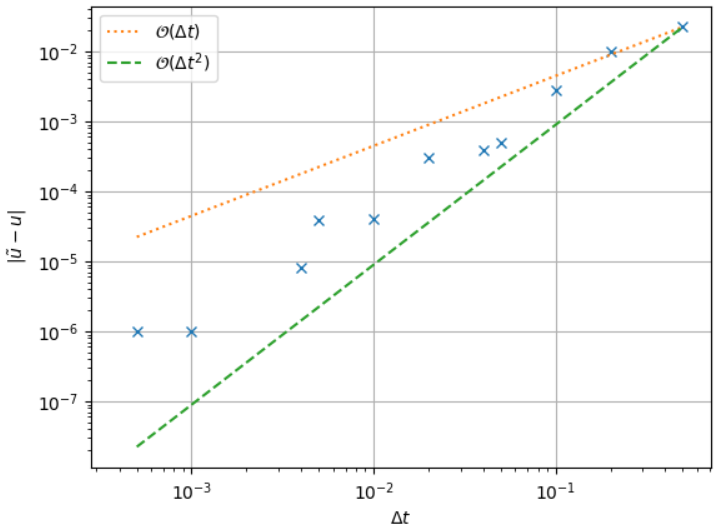
\includegraphics[width=\textwidth]{resources/calculix_convergence_study.png}
        \caption{}
    \end{subfigure}
    \hspace{0.8cm}
    \begin{subfigure}[b]{0.35\textwidth}
        \raisebox{0.11\height}{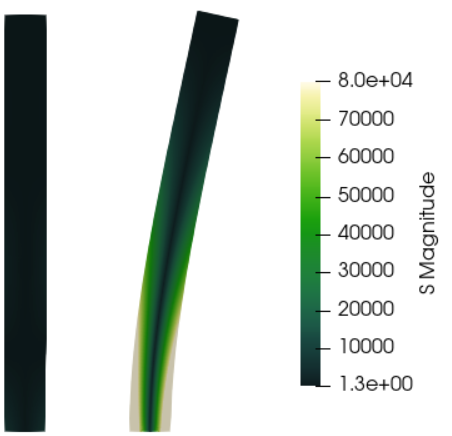
\includegraphics[width=\textwidth]{resources/elastic-flap.png}}
        \caption{}
    \end{subfigure}
    \caption{In Figure (a), we see the convergence study done over the displacement of the tip of an elastic flap, displaying a higher-order convergence.
    In Figure (b), we have an example of this elastic flap structural simulation, showcasing its elasticity. The colour scale represents the stress of the material.}
    \label{fig:calculix_convergence}
\end{figure}

Given the oscillatory behaviour of the flap, we measured the displacement of the flap's tip over time and used this value for the convergence study. As before, we implemented a script to automatize the execution of the simulations and the post-processing of the output data. We defined a reference solution $\tilde{u}$ as with the OpenFOAM study, which is the one obtained with a $\Delta t = 5\times 10^{-4}$. The output data format of CalculiX only has 6 significant digits, even though the solver works with double precision values. This means that we could obtain an output with better precision by modifying the solver's routines to export the data, but that rests out of the scope of this work. To circumvent this issue, we defined the simulation parameters so the error was significant enough to be visible in this precision range. This translates to a constant 10N force applied in the x-axis direction, and the measurements were taken at $t=2s$. Then, we plotted the absolute difference to the reference solution $|u - \tilde{u}|$ to observe how the error behaves relative to this solution. One can see in Figure \ref{fig:calculix_convergence} how the error decreases faster than $\mathcal{O}(\Delta t)$. With the obtained results, one can argue that the error follows a higher-order convergence, which in certain regions closely follows a second-order convergence. It is also noticeable how, for smaller timesteps, the error gets more oscillatory, which can happen due to the accumulation of other sources of error over time.


\section{Coupling the two solvers} \label{FSI_sec}

In the previous sections, we observed how a higher-order convergence is achievable with the OpenFOAM and CalculiX solvers. In this section, we will test them in a coupled simulation using the preCICE coupling library. To do so, we use the perpendicular flap setup found in the example tutorials of the library \cite{perpendicularFlap}. It consists of two components: a two-dimensional fluid flowing through a channel and a solid, elastic flap fixed to the floor of this channel. The fluid and solid parts of the simulation are computed by OpenFOAM and CalculiX, respectively, communicating between them with the help of preCICE. Figure \ref{fig:FSI} shows an example of this setup.

\begin{figure}[!ht]
    \centering
    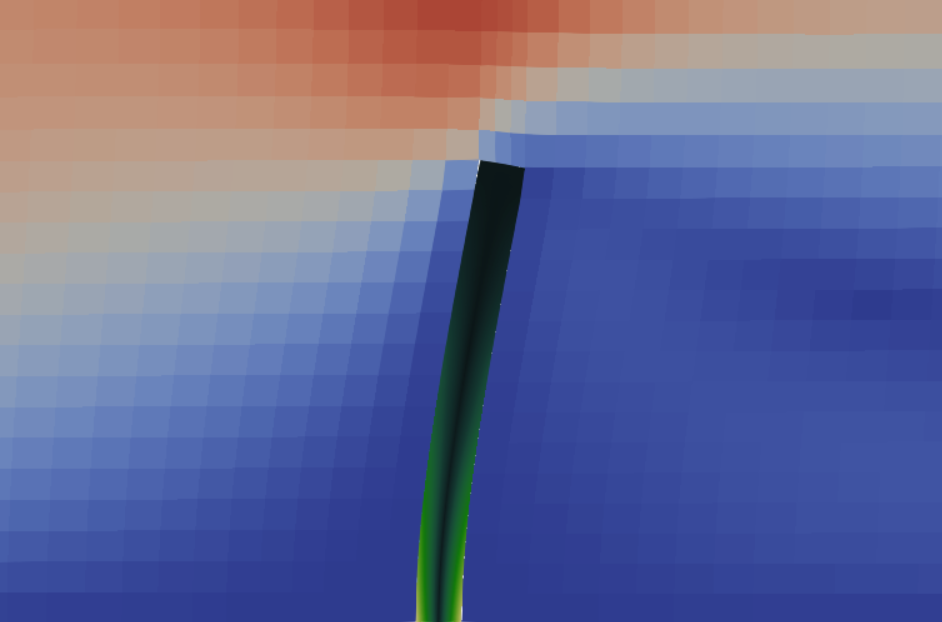
\includegraphics[width=0.45\textwidth]{resources/FSI_small.png}
    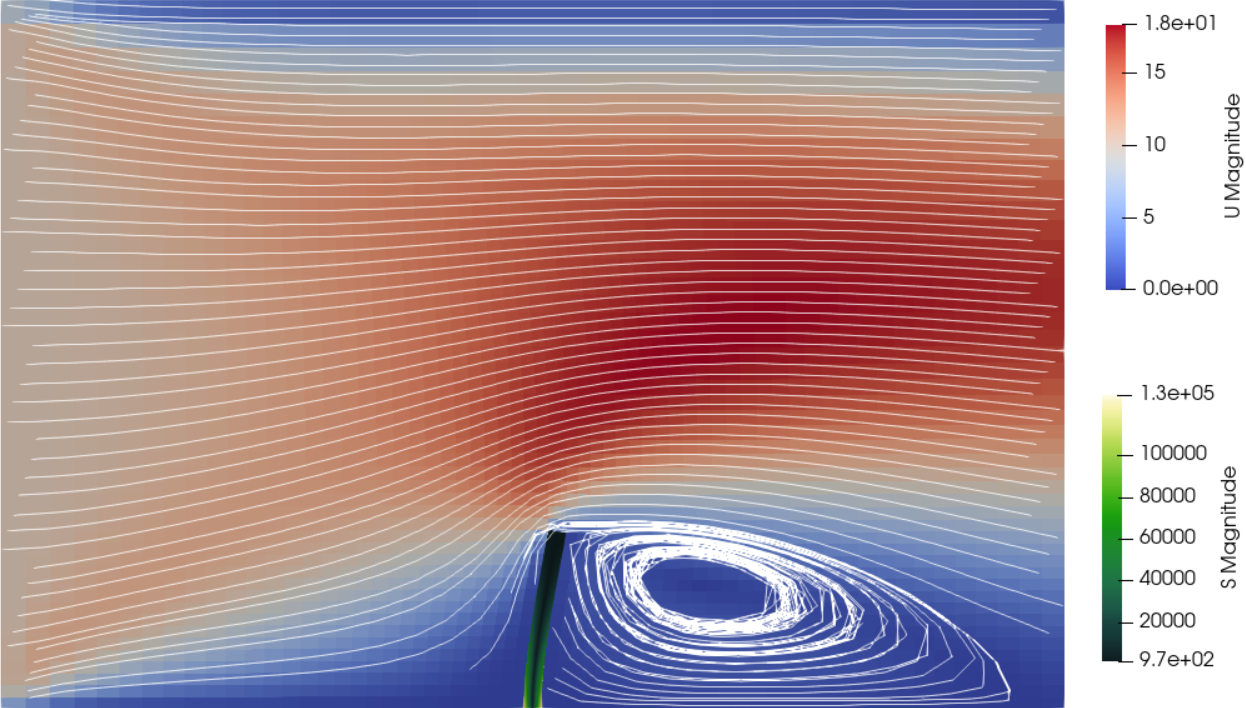
\includegraphics[width=0.53\textwidth]{resources/FSI_big.png}
    \caption{Example solution of the FSI simulation. The left image shows the zoomed-in flap, where the stress of the material can be seen on a green scale. In the right image, we observe the whole domain, where we see the magnitude of the velocity field.}
    \label{fig:FSI}
\end{figure}

The flap oscillates due to the fluid pressure building up on its surface during a limited period, given by its initial resting position. The oscillations dampen until the entire system reaches a steady state. We will quantify the simulation error by measuring the displacement of the flap tip at time $t=1s$, which is still in oscillatory behaviour. We wrote specific scripts once again to automatize this task, utilizing solver parameters similar to those in the previous sections. 

We ran multiple simulations, setting the same timestep size on both solvers and the preCICE configuration. We also used the Euler and Crank-Nicolson schemes, introduced in section \ref{sec:euler} for the fluid solver, to observe the difference in their error convergence. Moreover, we ran tests with the stable version 2 and the newest version 3 of preCICE to observe if the library update affected the overall error. 
\begin{figure}[!ht]
    \centering
    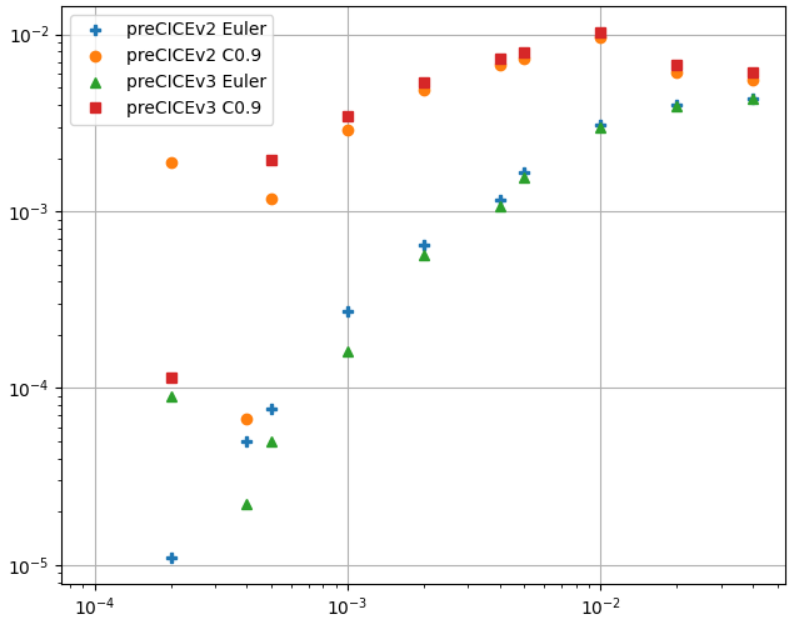
\includegraphics[width=0.5\textwidth]{resources/coupled_v2_v3_results.png}
    \caption{Convergence study of the coupled perpendicular flap scenario. The error is measured using the displacement of the tip and compared to a reference solution, which is the smallest computed value in each test. We repeated the same experiment using the Crank-Nicolson (CN) and the implicit Euler time stepping schemes. We also performed the same examples for the versions v2 and v3 of the preCICE library.}
    \label{fig:coupled_v2_v3}
\end{figure}

In Figure \ref{fig:coupled_v2_v3}, we can observe the results of this experiment. One can observe how we can achieve a first-order convergence of the error using the Euler method. Conversely, the Crank-Nicolson method performs poorly in this scenario, giving a worse convergence than the first-order method. It is relevant to mention how the different code versions give different results, even though it does not affect the convergence behaviour.

The reasons for the poor convergence of the second-order method can be various. preCICE is a complex environment with many moving pieces. Each solver has its adapter, which enables it to participate in a partitioned multi-physics simulation. This translates into many possible sources of error. In the following sections, we rule out possible sources of error and propose possible elements that could cause it.


\section{Possible sources of error}
This section aims to identify and address the potential sources of error we encountered while coupling OpenFOAM and CalculiX using the preCICE library. In section \ref{FSI_sec}, we observed that using a second-order time stepping method on the fluid solver gave worse error convergence than using a first-order scheme, despite both single solver analyses showing higher-order convergences. In this case, there are many possible sources of error, starting with the preCICE components. To ensure that the component to blame is not the solid participant, we will test its correct behaviour while coupled to a dummy implementation of the fluid participant. Moreover, we will also test the fluid participant in section \ref{sec:fluid-part}.


\subsection{Verification of CalculiX adapter}
PreCICE uses an adapter to interact with a participant solver, which serves as an interface between the solver and the preCICE library. To verify one of these adapters' correct behaviour, one can use a dummy implementation of another participant that only returns some preset magnitudes and couple both using preCICE.

To test the CalculiX adapter \cite{yau2016conjugate}, we implemented a fake fluid script that could be coupled with CalculiX using preCICE. This fake fluid \cite{pullrequestfake-fluid} participant applied a force on the flap with the direction of the positive x-axis, substituting what the OpenFOAM solver would produce on the FSI interaction. In this setup, the returned force by the fake fluid was not constant but varied over time, following $f^n = f_{max} \sin(t^n + \phi)$ on the tip and decreasing linearly over the height of the flap until reaching a 0 magnitude in the bottom. We aimed to approximate the forces applied by the fluid on the flap while making them time-dependent to observe a pronounced error decrease with a higher-order time stepping scheme.

\begin{figure}[!ht]
    \centering
    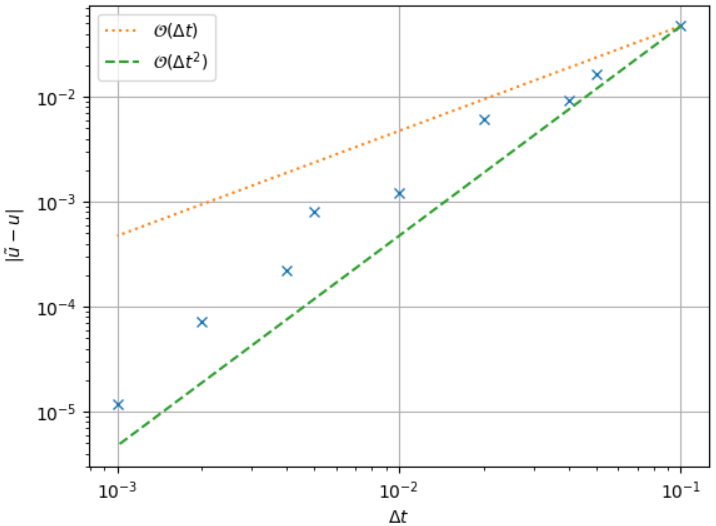
\includegraphics[width=0.5\textwidth]{resources/fake_fluid.png}
    \caption{Convergence study of the CalculiX adapter coupled with a fake fluid participant. The error is computed by measuring the displacement of the flap's tip and comparing it to a reference solution, which is the computed case with $\Delta t = 10^{-4}$. It displays a higher-order convergence in time.}
    \label{fig:fake-fluid}
\end{figure}

In Figure \ref{fig:fake-fluid}, one can observe that the error decreases in a higher-order fashion, as previously observed by the single solver study. This rules out this adapter as the possible source of error, as it shows good error convergence.

\subsection{Verification of fluid participant} \label{sec:fluid-part}
With the aim of verifying the fluid participant of the FSI simulation, we ran several single-solver simulations, only taking the fluid part of the scenario. The tested case could be seen as a channel with an inverse cavity that stands out, following the geometry of the flap. From this experiments, we observed that this setup was unstable for a high Courant–Friedrichs–Lewy (CFL) number, which is defined as $\text{CFL} = \frac{u \Delta t}{\Delta x}$. In the FSI simulation of section \label{sec:FSI}, we computed cases with a high CFL number when we had large timestep sizes, which failed to converge in this test. With the aim of improving the stability of the simulation we tried initializing the velocity field with precomputed values of a simulation that reached a steady state.

Once we could obtain some stable simulations, we defined a time-dependent input velocity to observe a decrease in the error when the timestep size was decreased. Then, a convergence study of the error was performed by running the same simulation with the Crank-Nicolson scheme and only varying the timestep size parameter. Doing this experiment, we could observe how the error did not follow a higher-order convergence. Its decreasing order was very similar to the one we observed in Figure \ref{fig:coupled_v2_v3} for the Crank-Nicolson scheme, which showcased that the fluid solver was the source of the poor error convergence.


\section{Conclusions and future work}
In this study, we examined the convergence behaviour of open-source solvers, specifically OpenFOAM and CalculiX, in single-solver and fluid-structure interaction (FSI) simulations using the preCICE coupling library. To do so, we developed a comprehensive pipeline to automate simulation execution and analysis, facilitating efficient exploration of various solver configurations. This allowed us to perform systematic convergence studies and to compare results across different scenarios. 

Our analysis yielded several key findings. OpenFOAM and CalculiX demonstrate the potential to achieve higher-order convergence when used independently on suitable scenarios and the correct solver configurations.
Moreover, we achieved a linear decrease in the error when using first-order time stepping methods on coupled simulations with preCICE. However, challenges arose in maintaining the higher order in FSI simulations. Through meticulous analysis and verification tests, we identified the fluid participant as the primary error source contributing to these discrepancies. Simultaneously, we verified the correct behaviour of the preCICE adapter for CalculiX. This reflected that the perpendicular flap scenario was inadequate to achieve a higher-order convergence with OpenFOAM. Some following work could be the thorough test of this setup utilizing other solvers that provide different higher-order time stepping schemes that are more robust than the Crank-Nicolson method. Exploring alternative physical configurations with lower CFL numbers would also be interesting, as it would provide better stability and facilitate the execution of convergence studies. Scenarios with finner spatial discretization could also help to observe a better error convergence, as the spatial error contribution would not be dominant until smaller scales. 

Overall, this study offers valuable insights into the convergence behaviour of open-source solvers and serves as groundwork for achieving more accurate coupled simulations.


\pagebreak

\printbibliography

\end{document}
